% Created 2021-05-15 sam. 14:39
% Intended LaTeX compiler: pdflatex
\documentclass[a4paper,12pt]{article}
\usepackage[position=top,labelformat=empty]{subfig}
\usepackage{caption}
\usepackage[hmargin=2cm,vmargin=3cm]{geometry}


\usepackage{amsmath}
\usepackage{graphicx}
\usepackage[boxed]{algorithm2e}
\usepackage{authblk,tikz}
\author[1,$\ddagger$]{Vaitea Opuu}
\author[1]{Nono S. C. Merleau}
\author[1]{Matteo Smerlak}
\affil[1]{Max Planck Institute for Mathematics in the Sciences, Leipzig, Germany}
\affil[$\ddagger$]{Contact email: vopuu@mis.mpg.de}
\date{\today}
\title{RNA fast-folding path for the prediction of secondary structures and folding dynamics}
\begin{document}

\maketitle
\begin{abstract}
The biological roles of non-coding RNA are better understood with
their structural features. The static structure predictions of RNAs have seen
tremendous progress in the thermodynamic and machine learning approaches. But an
understanding of dynamical aspects can provide for complementary biological
insights. Here, we propose a method to predict RNA structures and folding
dynamics. This method has been inspired by the RNA fast-folding paths principle.
For this, We developed an efficient algorithm exploiting the fast Fourier
transform and the stem rate model. It predicts multiple parallel folding paths
by following the thermodynamic energy landscape. When only a single prediction
per RNA was considered, this method's performance for the folding task was only
fair. However, when all structures found were analyzed, we found near-native
predictions (79\% PPV and 81\% sensitivity) for small RNA ($\lt$ 200
nucleotides). On average, those predictions were found to be of similar quality
to recent deep-learning-based methods. Furthermore, from these trajectories, we
built up a folding kinetic ansatz that allows extracting even more dynamical
information. Although only as few as $\sim$ 60 structures allowed us to produce
relevant folding kinetic trajectories while known methods may require millions
of them. Because of its simple foundations, this work can help develop new
insights into RNA structure roles.
\end{abstract}

\section*{INTRODUCTION}
\label{sec:org0105d5e}
Natural RNAs have various essential functions in many cellular contexts such as
in the protein translation machinery (mRNA, tRNA\ldots{})
\cite{ramakrishnan02_ribos_struc_mechan_trans}. In addition to its important place
in the central dogma of molecular biology, it also plays roles in gene
regulations (microRNAs) \cite{ambros04_funct_animal_micror}. In biotechnology,
RNAs also found its way with, for example, the design of biosensors or ribozymes
\cite{han10_desig_strat_aptam_based_biosen}. With ribozymes, RNAs entered the
realm of proteins where RNAs can perform enzymes functions. These functions are
generally understood through the lens of one static tri-dimensional structure.
This structure to function paradigm is used by most of the current frameworks to
understand relationships between RNAs. Since experimental determination of their
structures by X-ray or nuclear magnetic resonance are usually out of reach,
these analysis are based on predictions. Unfortunately, some important RNAs like
riboswitches have their biological function tightly bound to their dynamical
behavior \cite{vitreschak04_ribos}. A more complete description of RNAs static and
dynamical structural features is therefore desirable. And given the ever so
increasing number of RNA sequences, fast methods with such scopes could help in
tasks like refining data bases annotations. On the biotechnological side, such a
method could help develop new design strategies for synthetic RNAs
\cite{domin16_applic_comput_desig_approac_synth_ribos}.

Three main structure levels are generally considered to describe RNA molecules:
the primary structure is the nucleotide sequence itself. The secondary structure
is defined by interacting pairs of nucleobases called base pairs. The tertiary
structure involve other weaker non-trivial interactions within the same
sequence. Unlike proteins, RNA structures are usually hierarchically formed. The
secondary structure is formed first, followed by the tertiary structure
\cite{tinoco99_how_rna_folds}. Moreover, the secondary structure provides an
accurate enough description of the thermodynamics and kinetics of RNA molecules.
Although base pairs can be formed with various configurations
\cite{leontis01_geomet_nomen_class_rna_base_pairs}, we considered here only the
canonical base pairs edge-to-edge interactions: G-C, A-U, and G-U. Many formal
subtleties can be used to define the secondary structure, but we used here the
formal definition called pseudoknot-free. The important consequence is that each
base pair formed separates the RNA into two completely independent sections, the
interior and the exterior sections. In the rest of this work, structure refers
to the RNA secondary structure.

The structure space of an RNA molecule is described by the stability of all
possible structures. The stability \(\Delta G_s\) of a structure \(s\) is the free
energy changes with the completely unfolded state. To predict biologically
relevant structures, most of the current methods rely on free energy
minimization or stability maximization. The nearest-neighbor loop energy model
is the most used model to compute stabilities \cite{turner09_nndb}. By assuming
the additivity principle \cite{dill97_addit_princ_bioch}, the stability of a
structure is a sum of independent loop contributions. This model consists of a
set of tabulated parameter values associating free energy values to loop types
and nucleotide compositions. The Turner2004
\cite{mathews04_incor_chemic_modif_const_into} is one of the widely used set of
parameters. Its functional form allows for general energy parameters and the use
of an efficient dynamic programming algorithm. This algorithm can determine the
minimum free energy (MFE) structure of a sequence in the structure space. The
MFE is considered a gold standard for free-energy-based predictions, however, it
represents only one structural estimate among other. Other estimates exist such
as the maximum expected accuracy (MEA), however, it was not found to be
significantly better than the MFE \cite{mathews19_how_to_bench_rna_secon}.

Several tools implement the MFE search algorithm, namely Zucker algorithm
\cite{zuker81_optim_comput_foldin_large_rna}, such as \texttt{RNAfold}
\cite{hofacker03_vienn_rna_secon_struc_server}, \texttt{Mfold}
\cite{zuker03_mfold_web_server_nucleic_acid}, or \texttt{RNAstructure}
\cite{reuter10_rnast}. Although those methods were found to be consistently
accurate at predicting RNA secondary structures as shown in recent benchmarks
\cite{sato20_rna,huang19_linear}, the additivity foundation is expected to be
doomed when sequences get larger and structures complexify. Moreover, like
tertiary interactions, pseudoknots loop are not defined in the main parameters
sets like the Turner2004 model. The discrepancy for larger RNAs could be
explained by the fact that tertiary interactions and pseudoknots are neglected.
Machine learning (ML) approaches were investigated to overcome some of these
shortcomings. The ML structure estimate provides substantial improvements in
structure prediction according to recent benchmarks
\cite{singh19_rna_secon_struc_predic_using,sato20_rna}. But, in addition to some
over-fitting concerns \cite{rivas11_range_compl_probab_model_rna}, these
approaches cannot give dynamical information since too few data are available,
to this date, on structure dynamics. This structure estimate represents a
complex view of the RNA folding. Indeed, structural data are largely obtained
through phylogenetic analyses,

From a dynamical standpoint, the RNA molecule navigates the structure space by
following the landscape drawn by the stability. To follow the dynamic of
individual RNAs, three rate models describing elementary steps in the structure
space are currently used. First, the base stack model uses base stacks
formations and breaking as elementary moves \cite{zhang02_rna_hairp_foldin_kinet}.
The second model uses base pair as elementary steps. \texttt{kinfold}
\cite{flamm00_rna_foldin_at_elemen_step_resol} uses the base pair rate and a
continuous-time Monte Carlo simulation to follow the RNA folding dynamic. It
gives the finest resolution in the secondary structure folding landscape, but at
the cost of computation time. The third model uses the creation or deletion of
stems to construct the folding dynamics. It is the first strategy explored
\cite{martinez84_rna_foldin_rule}, and provides a coarse-grained description of
the dynamics. The folding rates are determined by the free energy changes when
stems are added or removed. Although none of these models were definitively
rejected nor accepted, this one makes a notable assumption. Indeed, transition
states (or saddle points) hidden in the formation of a given stem are not
considered \cite{zhang06_explor_compl_foldin_kinet_rna_hairp}. An alternative
approach, implemented in \texttt{kinwalker} \cite{geis2008folding}, used the observation
that folded intermediates are generally locally optimal conformations.
Therefore, locally optimal structures are formed using the standard dynamic
programming algorithm and aggregated together along with the folding procedure.

From folding experiments, Pan and coworkers found parallel pathways for a
ribozyme which involve two types of path to reach the native structure
\cite{pan97_foldin_rna_invol_paral_pathw}. One population of sequences was found
to fold rapidly, and one quickly reached metastable misfolded structures that
slowly fold into the native structure. However, in some cases, the metastable
states are functional, this is a direct consequence of the rugged nature of the
RNA folding landscape \cite{solomatin10_multip_nativ_states_reveal_persis}.
Russell and coworkers revealed experimentally the presence of multiple deep
channels separated by large energy barriers on the folding landscape which lead
to the fast and slow folding paths observed
\cite{russell01_explor_foldin_lands_struc_rna}. The formal description of this
mechanism, called kinetic partitioning mechanism, was introduced by Guo and
Thirumalai on proteins first \cite{guo95_kinet_protein_foldin}. In the free energy
landscape, those metastable conformations are competing attraction basins from
which RNA molecules are temporarily trapped.

Here, we propose a novel approach for RNA structure predictions and dynamics.
This method has been inspired by the fast-folding path idea and built upon
intuitive folding rules. The basic idea is to use the stem rate model to create
multiple parallel folding paths. It sequentially forms stems along the folding
trajectory if the stability is improved. Once a stem is formed, it cannot be
removed. To speed up the search of stems, RNA sequences are encoded in a
numerical fashion we called mirror encoding. This encoding combined with the
fast Fourrier transform allowed for a quick search of stems. This algorithm is
inspired by MAFFT \cite{katoh02_mafft}, a well-known multiple-sequence-alignment
tool. The use of signal processing techniques to analyze nucleotide sequences
has been investigated since the early 80's
\cite{felsenstein82_effic_method_match_nucleic_acid_sequen,benson90_fourier_method_bioseq_analy},
however, to our knowledge, this its first time use in an RNA folding algorithm.

To assess the reliability of the paths predicted, we compared its performance on
the folding task for a well-curated dataset, \texttt{ArchiveII}
\cite{mathews19_how_to_bench_rna_secon}. The algorithm predictions were compared
to two structure estimates: the MFE structure computed by \texttt{RNAfold} and the ML
structure computed with \texttt{MxFold2} \cite{sato20_rna}.

The low energy structure may not be the active structure. This can be explain by
the energy model limits but not only. Some RNAs may have their active structure
into kinetics traps far from the MFE. In some cases, the MFE may not even be
reachable in biologically relevant time. With the ensemble of paths produced for
each sequence, we also derived a folding kinetic ansatz. Next, we applied the
algorithm to a simple test case, the Coronavirus frameshifting stimulation
element \cite{baranov05_progr_ribos_frames_decod_sars_cov_genom}, and a classic
bi-stable sequence. These experiments allowed to find structures closer to the
native one for the biological first example. From the folding intermediates
obtained from RAFFT, we built a kinetic model from which we recovered
trajectories qualitatively similar to some trajectories obtained from the
barrier tree kinetic \cite{flamm02_barrier_trees_degen_lands}.

\section*{MATERIALS AND METHODS}
\label{sec:org005a1fa}
\subsection*{The folding algorithm}
\label{sec:org1684ddc}
We now describe the heuristic starting from one sequence of nucleotides
\(S=(S_1\dots S_L)\) of length \(L\), and its associated unfolded structure. We
first create a numerical representation of S where each nucleotide of \(S\) is
replaced by of one unit vector of 4 components:
\begin{equation}
\begin{split}
A \rightarrow \begin{pmatrix} 1\\ 0\\ 0\\ 0 \end{pmatrix},
U \rightarrow \begin{pmatrix} 0\\ 0\\ 0\\ 1 \end{pmatrix},
C \rightarrow \begin{pmatrix} 0\\ 1\\ 0\\ 0 \end{pmatrix},
G \rightarrow \begin{pmatrix} 0\\ 0\\ 1\\ 0 \end{pmatrix}.
\end{split}
\end{equation}
This gives us a (\(4 \times L\))-matrix we call \(X\) where each row corresponds to
a nucleotide type as shown below
\begin{equation}
X = \begin{pmatrix} X^A\\ X^C\\ X^G\\ X^U \end{pmatrix} = \begin{pmatrix} X^A(1) &X^A(2) &\dots &X^A(L) \\ X^C(1) &X^C(2) &\dots &X^C(L)\\ X^G(1) &X^G(2) &\dots &X^G(L)\\ X^U(1) &X^U(2) &\dots &X^U(L) \end{pmatrix}
\end{equation}
where, for example, \(X^A(i) = 1\) if \(S_i = A\). Next, we create a second copy
\(\bar{S}=(S_L\dots S_1)\) for which we reverted the sequence order. Then, each
nucleotide of \(\bar{S}\) is replaced by one of the following unit vectors:
\begin{equation}
\begin{split}
\bar{A} \rightarrow \begin{pmatrix} 0\\ 0\\ 0\\ w_{\scalebox{0.5}{AU}}\\ \end{pmatrix},
\bar{U} \rightarrow \begin{pmatrix} w_{\scalebox{0.5}{AU}}\\ w_{\scalebox{0.5}{GU}}\\ 0\\ 0\\ \end{pmatrix},
\bar{C} \rightarrow \begin{pmatrix} 0\\ 0\\ w_{\scalebox{0.5}{GC}}\\ 0\\ \end{pmatrix},
\bar{G} \rightarrow \begin{pmatrix} 0\\ w_{\scalebox{0.5}{GC}}\\ 0\\ w_{\scalebox{0.5}{GU}}\\ \end{pmatrix}.
\end{split}
\end{equation}
\(\bar{A}\) (respectively \(\bar{U}, \bar{C}, \bar{G}\)) is the complementary of \(A\)
(respectively \(U, C, G\)). \(w_{AU}\), \(w_{GC}\), \(w_{GU}\) are tunable parameters
that represent the weight associated with each canonical base pair. These
parameters are chosen empirically. We call this complementary copy \(\bar{X}\),
the mirror of \(X\).

To search for stems, we use the complementary relation between \(X\) and \(\bar{X}\)
with the correlation function \(\text{cor}(k)\). This correlation is defined as the sum
of individual \(X\) and \(\bar{X}\) row correlations
\begin{equation}
\text{cor}(k) = c_{X^A,\bar{X}^A}(k) + c_{X^U,\bar{X}^U}(k) + c_{X^G,\bar{X}^G}(k) + c_{X^C,\bar{X}^C}(k)
\end{equation}
where one row correlation between \(X\) and \(\bar{X}\) is given by
\begin{equation}
c_{X^\alpha,\bar{X}^\alpha}(k) = \frac{1}{\text{min}(k, 2 \times L-k)}\sum\limits_{\substack{1\leq i \leq L\\1 \leq i + k \leq L}} X^\alpha(i) \times \bar{X}^\alpha(i+k).
\end{equation}
For each \(\alpha \in \{A,U,C,G\}\), \(X^\alpha(i) \times \bar{X}^\alpha(i+k)\) is
non zero if sites \(i\) and \(i+k\) can form a base pair, and will have the value of
the chosen weight as described above. If all the weights are set to one,
\(\text{cor}(k)\) gives the frequency of base pairs for a positional lag \(k\).
Although the correlation requires \(O(L^2)\) operations, it can take advantage of
the FFT which reduces drastically its complexity to \(O(L\;\text{log}(L))\).

The large \(\text{cor}(k)\) values between the two copies indicate the positional
lag \(k\) at which the frequency of base pair is high. Indeed, this does not allow
to determine the exact stem positions. Hence, we use a sliding window strategy
to search for the largest stem within the positional lag. Since the copies are
symmetrical, we only need to slide over one-half of the positional lag. Once the
largest stem is identified, we compute the free energy change associated with
the formation of the stem. We perform the same search for the \(n\) highest
correlation values, which gives us \(n\) potential stems. Then, we fix into the
current structure the stem that give the best change of free energy. Here, free
energies were computed using Turner2004 energy parameters through Vienna RNA
package API \cite{lorenz11_vienn_packag}.

We are now left with two independent parts, the interior, and the exterior of
the stem formed. If the exterior part is composed of two fragments, they are
concatenated into one. Then, we simply apply recursively the same procedure on
the two segments independently in a "Breadth First" fashion to form new
consecutive base pairs. The procedure stops when no base pair formation can
improve the energy. Given this simple recursive scheme, it is straightforward to
consider pseudoknots by simply concatenating both parts. When multiple stems can
be formed in these independent fragments, we combine all the possible
independent stems and pick the composition that has the best overall stability.
If too many composition can be formed, we restrict this to the 10\textsuperscript{4} bests in
term of energy. Figure \ref{algo_desc} shows an example of execution to illustrate
the procedure. The complexity of this algorithm depends strongly on the number
and the size of the stems formed. The best case is the trivial structure
composed of one large stem where the complexity correspond to the correlation
evaluation for the whole sequence. The worst case is an idealized case where at
most \(L/2\) base pairs can be formed (assuming L is even). The rough complexity
depends on \(\sum \limits_{1\leq i \leq L/2} 2i \times \text{log}(2i) \approx
\frac{L^2}{2.} \times log(L) + \delta\) where \(\delta\) is small compared to
\(L^2\). Therefore, the procedure has a worst rough complexity of
\(O(L^2\;\text{log}(L))\).

The algorithm described so far tends to be stuck in the first local minima found
along the folding trajectory. To alleviate this, we implemented a stacking
procedure where the \(N\) best trajectories are stored in a stack and evolved in
parallel. Figure \ref{fast_path} illustrates this modified procedure. Like the
initial version, the procedure starts with the unfolded structure. Then, the
\(N=5\) best potential stems are stored at the first stack. From these \(N\)
structures, the procedure tries to add stems in the unpaired regions left and
save the \(N\) best structures formed. Once no stem can be formed, the algorithm
stops and output the structure with the best energy found among the structures
saved in the last stack. This procedure leads to the construction of a graph we
call fast-folding graph. In this graph, two structures are connected if the
transition from one to the other correspond to the formation of a stem.

\begin{figure}[htbp]
\centering
\includegraphics[width=.9\linewidth]{img/algo_img/fast_paths_graph.png}
\caption{\label{fast_path}\textbf{Fast folding graph derived from parallel folding paths.} In this example, the sequence is folded in two steps. The procedure starts with the unfolded structure in the left. \(N=5\) best stem formed are saved in the stack 1. From stack 1, multiple stems formation are considered, but only the \(N\) best are stored in the stack 2. Structures are ordered (from top to bottom) by energy in each stack. All the secondary structure visualization were obtained using VARNA \cite{darty09_varna}.}
\end{figure}

\begin{figure}[htbp]
\centering
\includegraphics[width=.9\linewidth]{./img/algo_img/algo_draw.png}
\caption{\label{algo_desc}\textbf{Algorithm execution for one example sequence which requires two steps.} (Step 1) From correlation (\(X, \bar{X}\)), we pick one peak which corresponds to a position lag. We search for the largest stem and form it. Two fragments, "In" and "Out", are obtained, but only the "Out" may contain a new stem to add. (Step 2) The procedure is call recursively on the "Out" sequence fragment only. It produces a new positional lag from which we form a new stem. The fragment left (colored in blue) do not contain any additional stem, so the procedure stops.}
\end{figure}

\subsection*{Kinetic ansatz analyses}
\label{sec:org8561e6e}
The folding kinetic ansatz used here is derived from the fast-folding graph. As
described in figure \ref{fast_path}, transitions can occur from left to right (and
right to left) but not vertically. Two adjacent structures \(x\) and \(y\) in this
graph are connected if the transformation from \(x\) to \(y\) (or \(y\) to \(x\)) only
requires the formation of a stem or if \(x\) and \(y\) are the same structure. The
fast-folding graph follows the idea that parallel paths quickly reach their end
points. If the end points are non-native states, those structures will slowly
fold back into the native state \cite{pan97_foldin_rna_invol_paral_pathw}. To
simulate this behavior, we use the population kinetics. As usually done, the
kinetic is modeled as a continuous time Markov chain
\cite{lorenz20_effic_comput_base_probab_multi_rna_foldin}, where populations of
structure evolve according to a network of structures and the transition rates
between structures. The fast-folding graph is used here as network of
structures. The Arrhenius formulation is commonly invoked to derive the
transition rates \(r(x \rightarrow y) \propto \text{exp}(-\beta E^{\ddagger})\)
where \(E^{\ddagger}\) is the activation energy separating \(x\) from \(y\), and
\(\beta\) is the inverse thermal energy (mol/kcal). However, here, we chose the
transition rates \(r(x\rightarrow y)\) to be based on the Metropolis scheme
defined as follow
\begin{equation}
r(x\rightarrow y) = k_0 \times \text{min}(1, \text{exp}(-\beta \Delta \Delta G(x\rightarrow y)))
\end{equation}
where \(\Delta \Delta G(x\rightarrow y)\) is the stability change between
structure \(x\) and \(y\). Therefore, this does not yield the traditional kinetic
analysis but an ansatz. \(k_0\) is a conversion constant that we set to 1 for the
sake of simplicity. This rate is non-zero if \(y\) is connected to \(x\) in the
graph (or \(y\) is in the neighborhood of \(x\), \(y \in \mathcal{X}\)). Here, we
initialize the population \(p_{0}\) with only unfolded structures, therefore, this
represents a complete folding mechanism. The population change of a structure
\(x\) is given by:
\begin{equation}
\frac{\text{d}p_x}{\text{d}t} = \sum_\limit{y \in \mathcal{X}}
r(y \rightarrow x) p_{y}(t) - r(x \rightarrow y) p_{x}(t)
\end{equation}
where the sum is running over the neighborhood \(\mathcal{X}\) of \(x\). \(p_{x}(t)\)
is the population of x at time \(t\).

\subsection*{Benchmark dataset}
\label{sec:orgf36bfba}
To build the dataset for the folding task application, we started from the
ArchiveII dataset. We first removed all the structures with pseudoknots since
all tools considered here don't handle pseudoknots. Next, we removed all the
structures which were evaluated with positive or null energy with the Turner2004
energy parameters. Since positive energies mean that the completely unfolded
structure is more stable than the native one. Those structures are assumed not
well modeled by the energy function used here and therefore would blur the
interpretation of the kinetic we try to extract. This dataset is composed of
2698 structures. 240 sequences were found multiple times (from 2 to 8 times). 19
of them were found with different structures. We discarded all duplication and
picked the structure with the lowest energy for each. We obtained a dataset of
2296 sequences.
\subsection*{Structure prediction protocols for benchmarks}
\label{sec:orgbe301a4}
To evaluate the structure prediction power of the proposed method, we compared
it to two structure estimates: the MFE structure, and one ML structure. To
compute the MFE structure, we used \texttt{RNAfold} with the default parameters and the
Turner2004 set of energy parameters. For the ML structure, we computed the
prediction using \texttt{Mxfold2} with the default parameters. Therefore, only one
structure prediction per sequence for those two methods were used for the
statistics.

Two parameters are critical for RAFFT, the number of positional lags in which
stems are searched and the number of saved configurations in the stack. For the
experiments, we search for stems in the 100 best positional lags and stored 50
conformations. The \(\text{cor}(k)\) which allow to choose the positional lags is
computed using the weights \(w_{GC}=3\), \(w_{AU}=2\), and \(w_{GU}=1\).

To compute the performance of RAFFT, we analyzed the output in two ways. First,
we only displayed the structure with the lowest energy found for each sequence.
Second, we compute the accuracy of all structures in the last stack predicted,
and displayed the best structure.

To measure the prediction accuracy, we used two metrics from epidemiology. The
positive predictive value (PPV) is the fraction of correct base pairs
predictions in the predicted structure. The sensitivity is the fraction of
correctly predicted base pairs in the true structure. Both metrics are defined
as follow
\begin{equation}
PPV = \frac{TP}{TP + FN}, \;\;\; \text{Sensitivity} = \frac{TP}{TP+FP}
\end{equation}
where TP, FN, and FP stand respectively for the number of correctly predicted
base pairs (true positives), the number of base pairs not detected (false
negatives), and the number of wrongly predicted base pairs (false positives). To
maintain consistency with previous and future studies, we computed these metrics
using the implementation in the \texttt{scorer} tool provided by Matthews and coworkers
\cite{mathews19_how_to_bench_rna_secon}, which provide also a more flexible
estimate where shifts are allowed.

\subsection*{Structure space visualization}
\label{sec:org632bee0}
To visualize the structure loop diversity in the ensembles of structures
considered here, we used the Principal component analysis (PCA). For one
ensemble of structure. We first extracted the loop compositions in percent for
each structure of the ensemble. To obtain the loop composition, we first convert
the structures into Shapiro notation using Vienna Package API. From the
notation, we extracted the sizes of interior, exterior, bulge, stacking,
hairpins, and multibranch loops. We obtain a table of 6 features and \(n\)
entries. This allows us to compute a \(6\times 6\) correlation matrix that we
diagonalize using the \texttt{eigen} routine implemented in the \(scipy\) package. For
visual conveniences, the structure compositions were projected onto the first
two principal components (PC). The direction of each feature in the PC space are
represented with arrows.

\section*{RESULTS}
\label{sec:org3ab19b4}
\subsection*{Application to the folding task}
\label{sec:org72156fe}
To evaluate the relevance of the folding method, we assessed its performance for
the folding task. Also, to measure the effect of sequence length, we analyzed
their performance length-wise. We compared the method with two structure
estimates: the MFE structure computed by \texttt{RNAfold} and the ML-based structure
computed by \texttt{MxFold2}. For RAFFT, we saved 50 structures for each sequence.

Figure \ref{perf_fig} A shows the performance in predicted positive values (PPV)
and sensitivity for the three methods. It shows that the ML method is
consistently better than RAFFT and MFE predictions, the thermodynamic methods.
The length-wise T-test between the MFE and ML predictions showed that this
difference is significant (p-value \(\approx\) 10\textsuperscript{-12}) with a substantial
improvement of about 10\%. Although RAFFT predictions were found to be comparable
to the MFE predictions, they are significantly less accurate (p-value \(\approx\)
0.0002), with a drastic loss of performance for sequences of length greater than
300 nucleotides.


\begin{table}[htbp]
\caption{\label{average_perf}Average performance in terms of PPV and sensitivity. First two rows shows the average performance for all the sequences per method. The lower two rows corresponds to the performances for the sequences of length \(\leq\) 200 nucleotides. RAFFT* correspond to the predictions where only the structures with the best accuracy was displayed.}
\centering
\begin{tabular}{llrrrr}
\hline
            &              & RAFFT & RAFFT* & MFE  & MLE\\
\hline
PPV         & All          & 47.8  & 59.7   & 55.9 & 70.4\\
Sensitivity & sequences    & 53.0  & 63.0   & 63.3 & 77.1\\
\hline
PPV         & sequences    & 58.2  & 79.0   & 59.5 & 76.7\\
Sensitivity & \(\leq 200\) & 63.6  & 81.6   & 65.5 & 82.9\\
\hline
\end{tabular}
\end{table}

Among the 50 structures saved per sequence with RAFFT, we found on average at
least one prediction with 59\% of PPV and 63\% of sensitivity as shown figure
\ref{perf_fig} A. The overall gain of performances is not significantly different
from the MFE predictions. However, for the sequences of length below 200
nucleotides, this gain was found to be substantial and significant (\(\approx\) 16 \%
better than the MFE) with PVV \(\approx\) 79\% and sensitivity \(\approx\) 81\%. The
accuracy for these predictions is equivalent to ML performances. For sequence
lengths greater than 300 nucleotides, we observed the same drastic loss of
accuracy, although we extracted the best prediction among the 50 saved
configurations for each sequence. We investigated the dependency to the base
pair spanning, however, we did not find any striking effect (see supp. mat.).

Two regions of lack of performance were observed for all methods. A group of 28
sequences of length shorter than 80 nucleotides have their known structures at
on average 9.8 kcal/mol greater than the MFE structures. Some of them involve
large unpaired loops such as displayed in figure \ref{perf_fig} B. The second
region is around 200 nucleotides in length. The known structure of these
sequences also displayed large unpaired regions (figure \ref{perf_fig} B).

To investigate the region of the structure space where the thermodynamic model
tends to fail, we extracted a view of the different structure space produced by
each method and the known structures. Figure \ref{perf_fig} C shows principal
component analysis (PCA) of the structure compositions in term of percent of
loops. From the PCA, we observed that the known structures are distributed in
the structure space toward interior loops. Also, some natural structures, as
shown in figure \ref{perf_fig} C, have large unpaired loops. The center of mass in
the principal component space is located in between the high-density stacking
and interior loops.

Next, we investigated the structure space produced by the three methods. The
thermodynamic approach seems to produce a more diverse structure space as shown
in figure \ref{perf_fig} D. Loop contents were extracted from the predicted
structures of each method and projected onto their respective two first
principal components space. Both RAFFT and MFE predictions seemed to produce
similar structure spaces. The ML method allowed for long unpaired regions such
as hairpins which tend to be closer to the structure space produced by the
dataset.

\begin{figure}[htbp]
\centering
\includegraphics[width=.9\linewidth]{img/illed_img/perf_illed.png}
\caption{\label{perf_fig}(A) Performance measured by PPV and sensitivity. RAFFT (blue) displayed the best energy found. RAFFT* (green) shows the best score found among the 50 saved structures for each prediction. The right pans of both figures show the distribution of PPV and sensitivity sequence-wise. (B) Structures found to be difficult to predict with the thermodynamic model. The sequence name where extracted directly from the dataset. (C) PCA analysis based on the native structures in the benchmark dataset. One example of structure found in the high density hairpins \textbf{H} is shown in the left. Both PCAs shows the same distribution, but on MFE (respectively RAFFT) shows in orange (respectively in blue) the structures with a PPV \(\leq\) \(10\%\). (D) The PCA for the predicted structures obtained with all three methods.}
\end{figure}

\subsection*{Selected applications of the kinetic ansatz}
\label{sec:org20ac1ca}
The active structure observed is, in some cases, in kinetic trap far from the
MFE on the free energy landscape. To illustrate those phenomenon, we applied
folding kinetic ansatz proposed to two RNAs: the Coronavirus frameshifting
stimulation element and one classic bi-stable sequence. The Coronavirus
frameshifting stimulation element is an RNA sequence of about 82 nucleotides
with a secondary structure determined by sequence analysis and obtained from the
RFAM database. The known structure has a pseudoknot but was not taken into
account here. Figure \ref{test_case} panel A and B show the fast-folding graph,
the MFE prediction, and the known structure. The folding mechanism is predicted
in at most four steps where 20 structures were stored and 100 positional lags
were searched for stems. RAFFT was able to recover near-native structures, found
to be closer than the MFE. Nevertheless, The greediness effect can be easily
spotted at step two in the fast-folding graph. One intermediate leading to the
MFE structure is ranked 9. Hence, if less than 9 structure are stored, the MFE
structure cannot be obtained.

To visualize the folding landscape drawn by RAFFT, we mapped all 68 unique
structures found onto a plan using the multidimensional scaling (MDS) algorithm.
On this landscape, the MDS optimized the mapping in such a way that the
structure base pair distances are mostly preserved. Figure \ref{test_case} panel D
shows the landscape interpolated with the unique structures found. It
illustrates the two states folding landscape where all trajectories started from
the high peak in the center, and smoothly roll down to the good stability area
(blue area).

Figure \ref{test_case} shows the kinetic obtained from the fast-folding graph. The
near-native structure 44 dominates the kinetic between t=10\textsuperscript{2} to t=10\textsuperscript{13}. Its
stability was evaluated at -23.2 kcal/mol. Then, one of the MFE structures
dominated the population from t=10\textsuperscript{13} to the t=10\textsuperscript{15} and has been evaluated with
a stability of -25.8 kcal/mol. As shown in figure \ref{test_case}, long-live
intermediates are structures that couldn't be folded any further, such as
structures 25, 27, 28, or 30. One speculative folding scenario that may support
this kinetic model is the formation of the pseudoknot when the structure 44
dominates the population, which may have fixed the observed secondary structure.

\begin{figure}[htbp]
\centering
\includegraphics[width=.9\linewidth]{img/test_case.png}
\caption{\label{test_case}(A) Fast-folding path in four steps and 20 saved structures. The edges are colored according to the \(\Delta \Delta G\) of stability. At each step, the structures are ordered by their stability from top to bottom. The minimum energy structure found is at the top left of the graph. Visited structures in the kinetic are annotated by a unique ID. (B) MFE (computed with RNAfold) and the native structures of the Coronavirus frameshifting element. (C) Kinetic of structures with an arbitrary time. (D) Folding landscape derived from the 68 unique structures found by RAFFT. The axes are the components optimized by the MDS algorithm so the base pair distances are mostly preserved. Observed structures are also annotated using the unique ID. The MFE like structures (\textbf{MFE.l}) are in the bottom of the figure while the native like (\textbf{Nat.l}) are in the top.}
\end{figure}

Next, we compared the fast-folding kinetics with the widely used barrier tree
kinetics \cite{flamm02_barrier_trees_degen_lands}. First, we generated the \(1.5
\times 10^6\) suboptimal structures at 15 kcal/mol from the MFE structure using
\texttt{RNAsubopt} \cite{lorenz11_vienn_packag}. Since the MFE structure is evaluated at
-25.8 kcal/mol, the unfolded structure couldn't be sampled. Next, the ensemble
has been coarse-grained into 40 basins and presented as a barrier tree in figure
\ref{treekin} A. Here, the kinetics represent the competition between basins. The
coarsening was performed by the tool \texttt{barrier}
\cite{flamm02_barrier_trees_degen_lands}. The barrier tree displayed a bi-stable
topology. The near-native structure is the deepest basin in the lower part of
the tree (its structure ID is 4). From the barrier tree and the Arrhernius
formula \cite{wolfinger04_effic_comput_rna_foldin_dynam}, we used the tool
\texttt{Treekin} to derive transition rates and compute folding kinetics. Since the
unfolded structure couldn't be reached, we chose two other structures to
initialize two kinetic trajectories (structures I1 and I2). Figure \ref{treekin} C
shows the folding kinetic where the near-native and MFE structures are
dominating the population at different interval such as displayed by
fast-folding kinetic model in figure \ref{test_case}. When the trajectory was
initialized in the same branch than the MFE, the simulation is directly
dominated by the MFE after t=10\textsuperscript{1}.

\begin{figure}[h!]
\centering
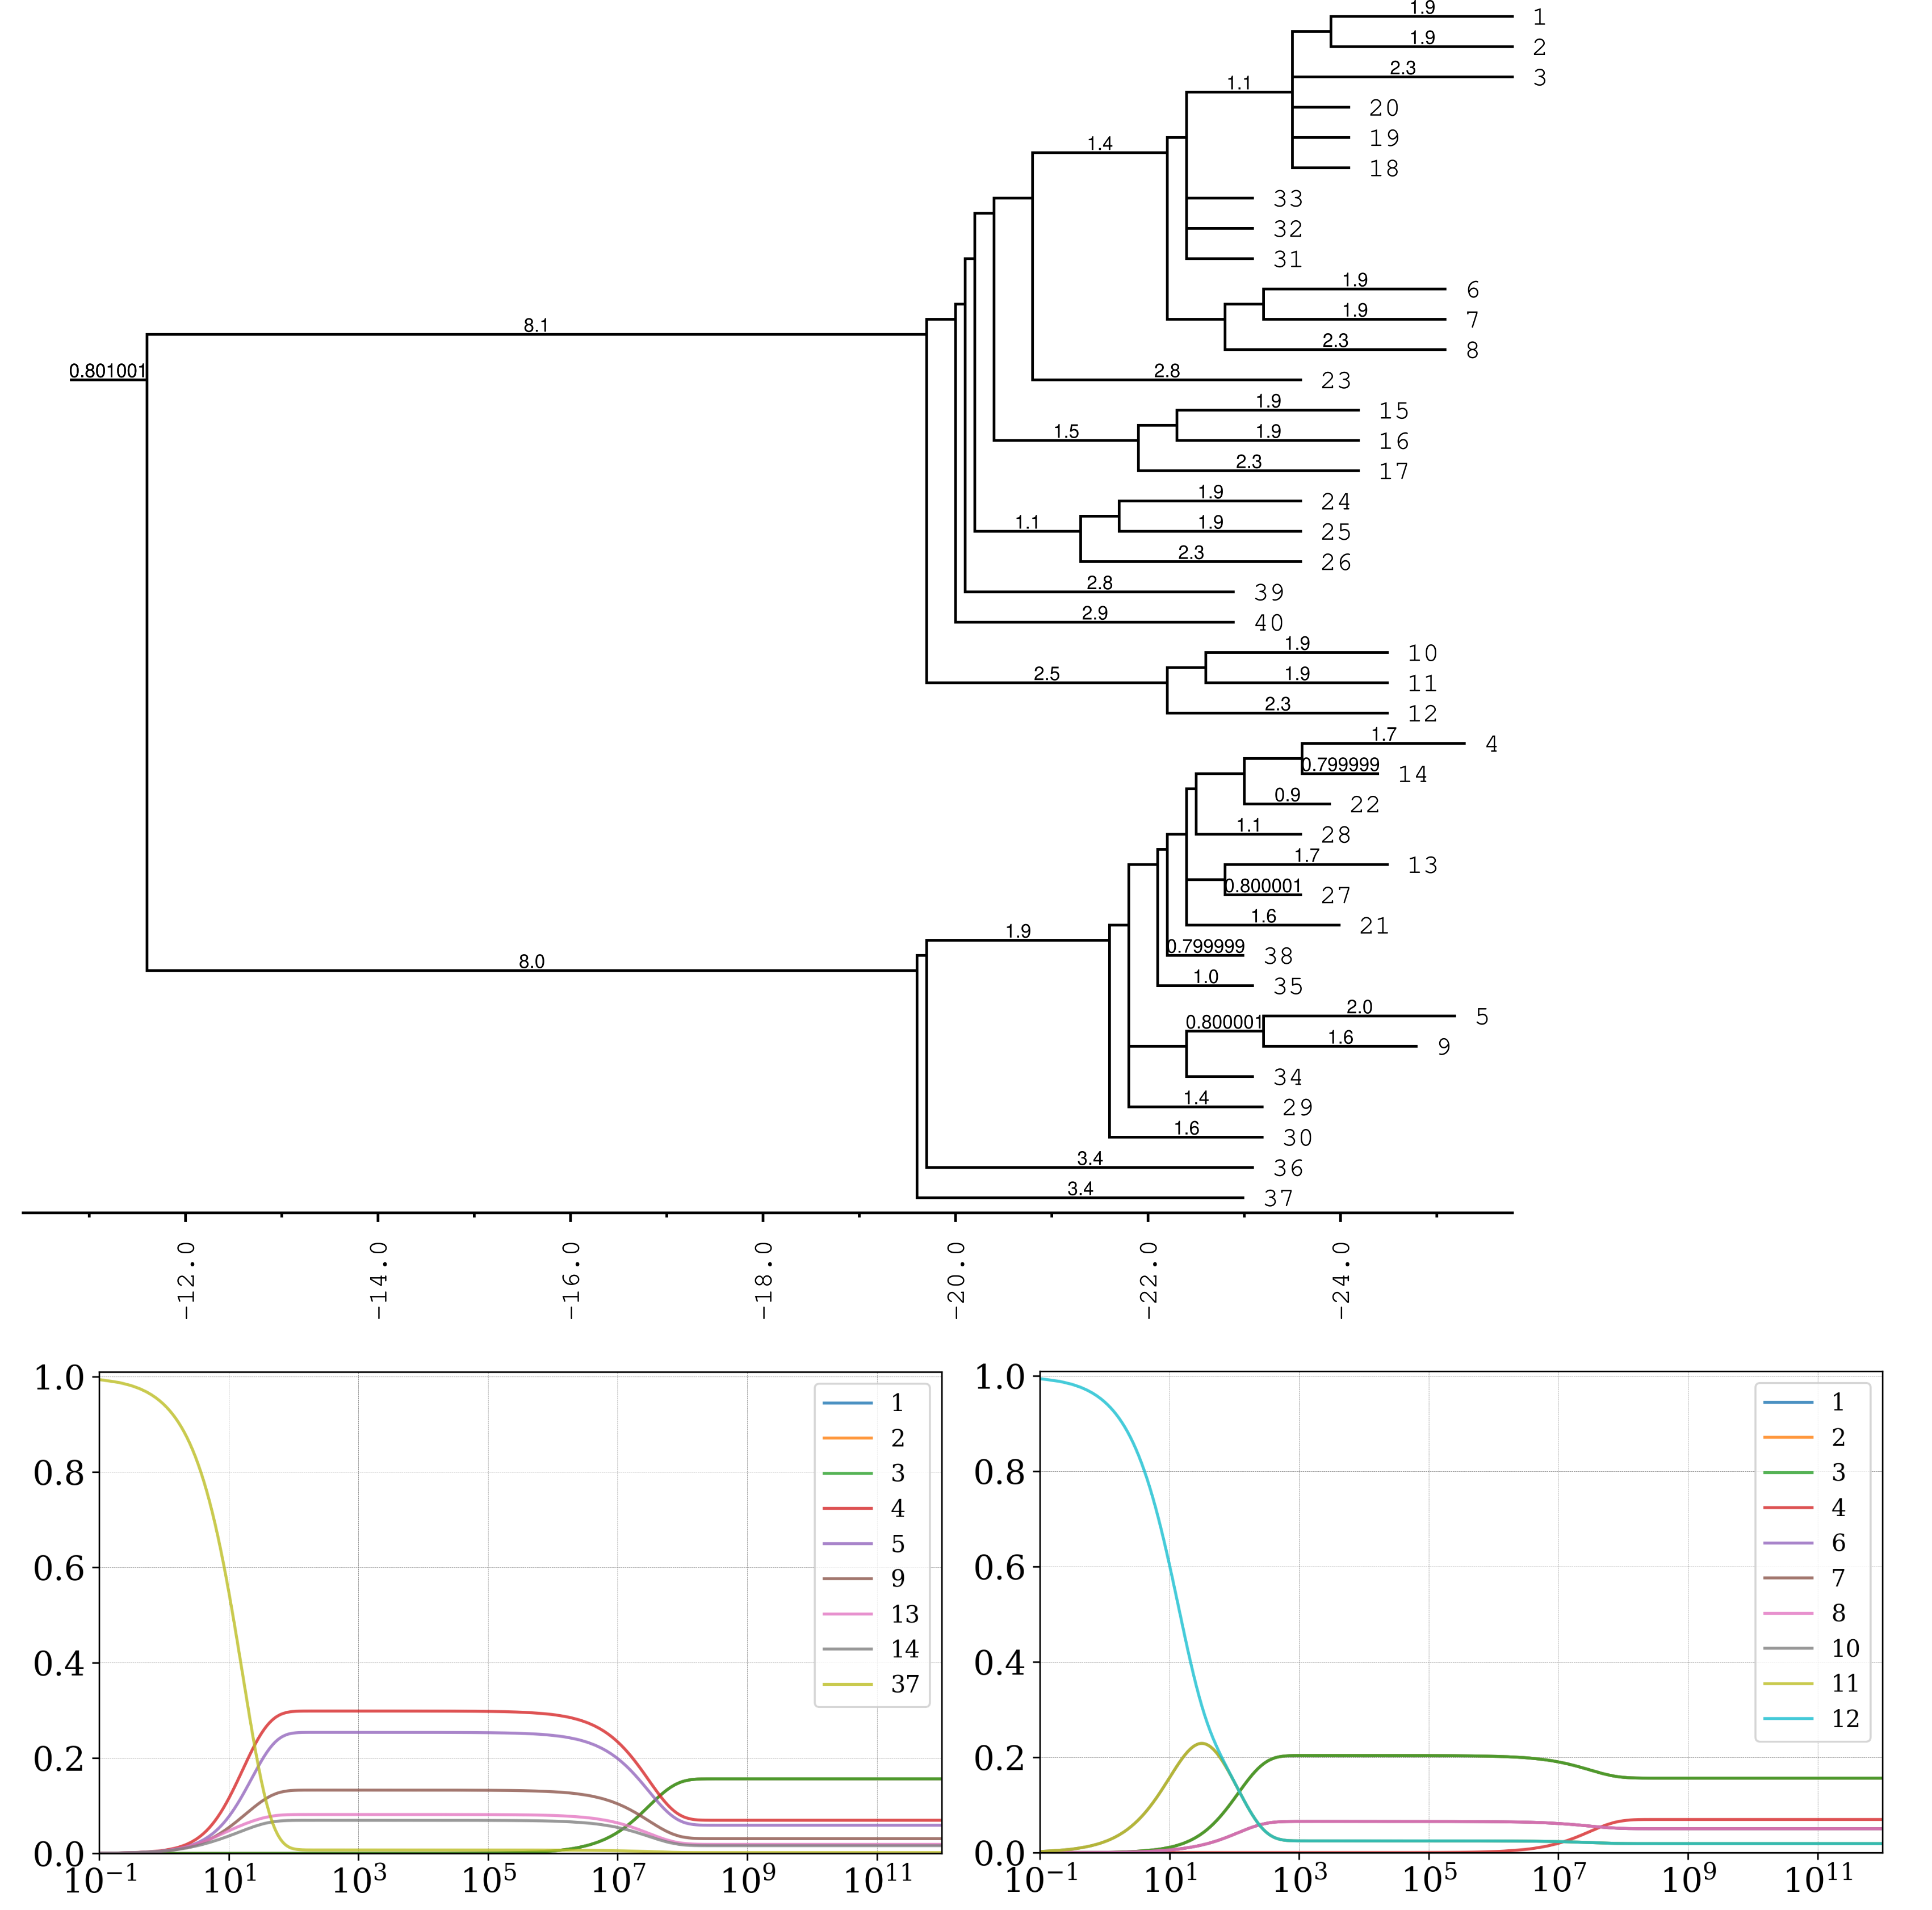
\includegraphics[width=.9\linewidth]{img/kinetic_treekin/kinetic_treekin.png}
\caption{\label{treekin}(A) Barrier tree obtained for the Coronavirus frameshifting element. (B) Kinetics where the initial population started with structure I1. (C) Kinetics where the initial population started with structure I2.}
\end{figure}

To further investigate the fast-folding kinetics, we tested a classic bi-stable
example, the sequence \texttt{GGCCCCUUUGGGGGCCAGACCCCUAAAGGGGUC}. Because of its
length, we were able to sample the whole space of sub-optimal structures from
the unfolded state to the MFE structure. The ensemble is composed of \(20 \times
10^3\) structures. The barrier tree derived from this ensemble displayed the
bi-stable system. The two relevant structures are denoted SA and SB (figure
\ref{class_examp}). If initialized in the lower part of the tree, the kinetic
produced is similar to the one obtained with RAFFT. First, the SB structure
dominated the population from t=10\textsuperscript{2} to t=10\textsuperscript{10}, then the SA structure took over
the population. Otherwise, if the kinetic is initialized in the other basin,
only the MFE dominated the population.

\begin{figure}[h!]
\centering
\includegraphics[width=.9\linewidth]{img/kinetic_treekin/kine_bi_sta.png}
\caption{\label{class_examp}(A) Barrier tree for the sequence \texttt{GGCCCCUUUGGGGGCCAGACCCCUAAAGGGGUC}. (B) Left side is the kinetic trajectory when initialized with structure 22. (B) Right size is the kinetics trajectory when initialized with structure 26. A') The fast folding paths with 20 saved structures and 100 stem searched. B') Fast-folding kinetic trajectory obtained from the bi-stable system (indices are different from the barrier tree indices).}
\end{figure}

\section*{DISCUSSION}
\label{sec:orgedf3722}
We have proposed a heuristic of the RNA structure and dynamic predictions called
RAFFT. This heuristic uses simple folding rules based on the stem rate model.
First, it searches for groups of consecutive base pairs, stems, and form them if
they improve the stability. We implemented an FFT-based technique that uses a
mirror encoding to quickly identify stems. Once a stem is formed, the sequence
is split into two independent parts on which the procedure is recursively
called. To mimic the parallel folding paths naturally observed, we implemented a
stacking procedure where multiple parallel folding trajectories can be stored.

To assess the relevance of the folding trajectories produced, we compared the
algorithm performance for the folding task. Two structure estimates were
compared with: the MFE structure computed using \texttt{RNAfold}, the ML estimate using
\texttt{MxFold2}. Other thermodynamic-based and ML-based tools were investigated but
not shown here. We chose the MFE since it provides an intuitive interpretation
in the structure landscape. The ML estimates gives a data view of the structure
spaces. Although, it has better prediction accuracy, it also include signal from
other folding mechanism such as the effects of chaperon proteins. Therefore, the
ML estimate may include effects that are induced by the environment of those
RNAs.

From our experiments, RAFFT had an overall performance below the MFE predictions
by 8.1\% of PPV and 10.3\% of sensitivity. The ML-based approach dominated the
predictions (70.4\% of PPV and 77.1\% of sensitivity). We observed some drastic
loss of accuracies when the known structures contained large unpaired regions.
However, those sequences were anecdotal in the dataset. Moreover, those regions
are unlikely to be stable and assumed to be very flexible. Nevertheless, the
effect of unpaired regions seemed less dramatic for the ML method since it can
produce some of those atypical structures. We found no striking evidences of the
length effect on prediction quality. In addition, no empirical effects of the
base spanning was observed (see supp. mat.) as already pointed out in
\cite{amman13_troub_long_range_base_pairs_rna_foldin}.

The PCA performed on the known structure compositions revealed a structure space
prone to elongated structures where large unpaired hairpin loops and exterior
loops can be observed. The PCA analysis performed on the structures predicted by
the thermodynamic-based methods (RAFFT and MFE) shown similar structure spaces,
where unpaired regions are of limited number. On the other hand, the ML method
seemed to be closer to the natural structure space. According to the
thermodynamic model, those unpaired regions have local stability equal to zero.
Hence, those regions are not stable at regular experimental conditions in the
sense that they may not have a unique stable structure. However, the ML-method
was able to identify such structure more consistently than thermodynamic
methods. This PCA revealed a group of structures with high percents of hairpins.
This may suggest some overfitting effects.

Although the overall performance of RAFFT was only fair in the folding task, we
found one among the \(k=50\) predicted trajectories that had better accuracy than
the low energy structure displayed. In fact, the gain of performance is
substantial for the sequences of length below 200 nucleotides with 16\% gain in
PPV compared to the MFE predictions. The performance is similar to the ML-base
method for this length range. Sequences of length \textless{} 200 nucleotides represent
86.4\% (1983 sequences) of the total dataset. This shows that some of folding
scenarios in all parallel folding path stored by RAFFT are relevant.

For the 140 sequences of length greater than 300 nucleotides, all 50 predictions
per sequence performed worst than the other methods. This could be partially
explained by the greediness of the algorithm, however, we also believe that the
energy model assumption such as the additivity could give a complementary
explanation \cite{tinoco99_how_rna_folds}. However, the MFE did not show any
notable discrepancy for large sequences (\textgreater{} 300 nucleotides) except for a few
structures with large unpaired regions. This could be explained by the
observation used in \texttt{kinwalker} where locally optimal substructures composed the
native structures. Therefore, the MFE structures may be more often composed of
locally optimal structures. We tried RAFFT with a larger number of saved
structures in the stack, however, it only got closer to the MFE prediction
quality and did not perform better on large sequences (see supp. mat.).

As an illustrative example, we applied our method on a natural RNA and a classic
toy system. The folding trajectories produced by RAFFT started from the
completely unfolded state and depicted simple "two-states" folding mechanisms.
We showed that these fast-folding graphs obtained from RAFFT can be used to
derived kinetic ansatz. Usual kinetic frameworks
(\cite{lorenz20_effic_comput_base_probab_multi_rna_foldin}) involve the sampling
of many thousands of structures then a coarse-grain procedure into basins. Then,
an arbitrary choice of initialization is needed to simulate the structure
competition. Here, since all folding graphs started from the completely unfolded
structure, the proposed kinetic model can describe the complete folding process.
When compared to the fast folding kinetics, we obtained similar results for some
chosen initial conditions.

Given the results, we believe that RAFFT is a robust heuristic for the structure
predictions since it can predict structure of high accuracy for 86.4\% of this
dataset. The folding paths as calculated by RAFFT are intuitive and
coarse-grained since whole stems are formed sequentially. The folding landscape
depicted by the proposed method also get along with the traditional two-states
protein folding model. Furthermore, the proposed kinetic ansatz derived from the
fast-folding graph was shown to approximate well the usual kinetic framework but
with a gain in the number of structure needed. However, additional efforts are
necessary to determine whether the folding paths followed were experimentally
observed and when this folding model is likely to fail.

On the technical points, the mirror encoding as describe here is a versatile
tool for RNA analysis. Since it contains the relative positions of base pairs in
the whole sequence, we expect it to be extendable to other use cases such as
sequence clustering, or the speed up of Nussinov-like algorithms. On the other
hand, we are aware of the limits of choosing the largest stem at each step and
will exploring different schemes. However, the greediness of the algorithm had a
limited impact on the results. Another limit of the method is the choice of the
relevant path among all parallel path predicted for one sequence. To alleviate
this, we propose to compute ML-based scores to determined which structure is
likely to be observed among the \(N\) saved structures by RAFFT.

\section*{DATA AVAILABILITY}
\label{sec:org95f7fbb}
One implementation in \texttt{python3.0} of RAFFT and the benchmarck data used in this
manuscript are available from \url{https://github.com/strevol-mpi-mis/RAFFT}. We also
provide the scripts used for the figures and kinetic analyses.

\section*{FUNDING}
\label{sec:orgc13f55b}
\section*{ACKNOWLEDGEMENTS}
\label{sec:orgbb01ba4}

\bibliographystyle{acm}
\bibliography{d1}
\end{document}
